\scanpage{15}
Les deux pts isotropes (confondus \deleted{\unsure{sur}} en \unsure{la|chaque} fibre en un $s$ sss $\alpha_s=\deleted{\unsure{+}}-2\ldots$) correspondent aux \deleted{solutions} directions de pente $\unsure{\zeta|\xi}=y/x$ satisfaisant
\[
\zeta^2-\alpha\zeta+1=0\qquad\text{i.e.}\qquad\zeta+\zeta^{-1}=\alpha
\tag*{(7)}
\]
Étudions la situation où on se donne (en plus du polygône épinglé) une telle direction isotrope -- ici le \deleted{schéma} ``module'' est donc \inserted{la section inversible} $\zeta$, plus fin que $\alpha$ [et pour les \deleted{\unsure{ép}} ``$n$-polygônes'' on aura $\Phi_n(\zeta)=0$ \margin{pol. cyclotomique} $+$ condition de caractéristique...] Donc la forme quadratique $q_0$ s'écrit
\[
q_0(x,y)=(x\unsure{-}\zeta y)(x-\zeta^{-1}y)
\tag*{(8)}
\]
et $q(x,y,z)$ s'écrit
\[
q(x,y,z)=(x-\zeta y)(x-\zeta^{-1}y)-(x+y)z
\tag*{(9)}
\]
Utilisons \deleted{\unsure{$\zeta$}} la \deleted{droite du}\inserted{droite $D_\zeta$ de pente $\zeta$ et} le pt isotrope $d_\zeta\in C$ \deleted{de pent\unsure{e} $\zeta$}\inserted{correspondant} pour identifier la cônique $C$ : $q(x,y,z)=0$ à $\mathbb P(E/D_\zeta)$ -- on trouve

\figure{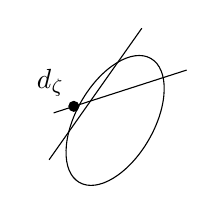
\begin{tikzpicture}[x=.64cm,y=.64cm]
\draw[rotate around={-30:(0,0)}] (0,0) ellipse (.77 and 1.42);
\draw (-1.31,-.78)--(.53,1.83);
\draw (-1.22,.15)--(1.42,1.00);
\fill (-.82,.28) circle (2pt) node[above left] {$d_\zeta$};
\end{tikzpicture}}
Un \unsure{répère|repère} projectif de $\mathbb P(E/D_\zeta$ \unsure{grace|grâce} aux trois plans suivants contenant $D_\zeta$ i.e. aux droites projectives de $\check{\mathbb P}(E)$ contenant $d_\zeta$

\unsure{0)|a)|$\circ$)} \deleted{le plan qui \unsure{correspond}}\inserted{celui qui correspond} la droite tangente à $d_\zeta$ à $C$
% archive sheet number: 14
